\section{Introduction}
\begin{frame}
\frametitle{Edit Operations\ldots}
\begin{itemize}
  \item \ldots define \textbf{Building Blocks} of (common) changes
  \item \ldots are specified as a \textbf{rule}, defining:
  \begin{itemize}
    \item  (Parameterizable) Context
    \item Changes to apply
    \item Application Conditions
\end{itemize} 
  \item \ldots can be used for:
  \begin{itemize}
    \item Differencing
    \item Patching
    \item Merging
    \item Refactoring
    \item \ldots
    \end{itemize}
\end{itemize} 
\end{frame}

\begin{frame}[t]
  \frametitle{Use Case: Model Evolution}
  \begin{center}
  \includegraphics[width=0.9\textwidth]{images/uml_example_05_01}
  \end{center}
\end{frame}
\begin{frame}[t,noframenumbering]
  \frametitle{Used Edit Operation}
  \begin{center}
  \includegraphics[width=0.9\textwidth]{images/uml_example_05_02}
  \end{center}
\end{frame}

% \begin{frame}
% \frametitle{SiLift on one Slide}
% \begin{columns}[t]
% \begin{column}{0.5\textwidth}
% \begin{block}{Differencing}
%   \begin{center}
% \includegraphics[scale=0.47]{images/createPatch}
%   \end{center}
% \end{block}
% \end{column}
% \begin{column}{0.5\textwidth}
% \begin{block}{Patching}
%   \begin{center}
% \includegraphics[scale=0.41]{images/applyPatch}
%   \end{center}
% \end{block}
% \end{column}
%  \end{columns}
% \begin{block}{Merging}
%   \begin{center}
% \includegraphics[scale=0.55]{images/applyPatchMerge}
%   \end{center}
% \end{block}
% \end{frame}

\begin{frame}
  \frametitle{Edit Operation - Implementation}
  \begin{center}
  \includegraphics[scale=2.0]{images/henshinLogo}\\
  \includegraphics[scale=0.3]{images/pullUp_HR}
  \end{center}
\end{frame}

% \begin{frame}[t]
%   \frametitle{Model Evolution}
%   \begin{flushleft}
%   \includegraphics[scale=0.46]{images/uml_example_01}
%   \end{flushleft}
% \end{frame}
% 
% \begin{frame}[t,noframenumbering]
%   \frametitle{Model Evolution}
%   \begin{flushleft}
%   \includegraphics[scale=0.46]{images/uml_example_02}
%   \end{flushleft}
% \end{frame}
% 
% \begin{frame}[t,noframenumbering]
%   \frametitle{Model Evolution}
%   \begin{flushleft}
%   \includegraphics[scale=0.46]{images/uml_example_03}
%   \end{flushleft}
% \end{frame}
% 
% \begin{frame}
%   \frametitle{Model Evolution}
%   \begin{center}
%   \includegraphics[scale=0.4]{images/uml_example_04}
%   \end{center}
% \end{frame}
% 
% \begin{frame}
%   \frametitle{What textual difference tools report\ldots}
%   \begin{center}
%   \includegraphics[scale=0.55]{images/text_compare}
%   \end{center}
% \end{frame}
% 
% \begin{frame}
%   \frametitle{What EMFCompare reports\ldots}
%   \begin{center}
%   \includegraphics[scale=0.55]{images/emf_compare}
%   \end{center}
% \end{frame}

% \begin{frame}
%   \frametitle{What SiLift reports\ldots}
%   \begin{center}
%   \includegraphics[scale=0.5]{images/symmetric_collapsed}
%   \end{center}
% \end{frame}